%9 Thanks to: https://tex.stackexchange.com/q/565173/64425
\documentclass[a4paper, 12pt]{article}
\usepackage{geometry}
\geometry{
    bottom=20mm,
    left=20mm,
    right=20mm,
}

\usepackage{polyglossia}
\usepackage{fontspec} % only for direct unicode codepoint interpretation
\usepackage{makecell}
\usepackage{graphicx}
\usepackage{longtable}
\setdefaultlanguage{english}
\setotherlanguages{sanskrit}
\setmainfont[Language=English]{IBM Plex Sans}
% Other font (for Sanskrit): Shobhika
\newfontfamily\sanskritfont[Mapping=velthuis-sanskrit,Script=Devanagari,Language=Default]{Shobhika}
\newcommand \sansletter[1]{
    \fontsize{2cm}{2.4cm}\selectfont
    \sans{#1}
}
\usepackage{xcolor}
\newcommand\TODO[1]{\colorbox{red}{#1}}
\usepackage{footnote} % for footnotes in tables, tabulars
% stack characters vertically
\usepackage{stackengine,scalerel}
\newcommand\mystack[2]{\scaleleftright{.}{\Shortstack{#1}}{#2}}
\setstackgap{S}{0pt}
% stack characters vertically
\usepackage{hyperref}
\hypersetup{
    colorlinks=true,
    linkcolor=blue,
    anchorcolor=brown,
    citecolor=blue
}
\newcommand \eng[1]{
    \textenglish{#1}
}
\newcommand \sans[1]{
    \textsanskrit{#1}
}
\newcommand \shortsansletter[1]{
    \textcolor{red}{\sansletter{#1}}
}
\newcommand \longsansletter[1]{
    \textcolor{blue}{\sansletter{#1}}
}
\newcommand \sansconsonant[1]{
    %\textcolor{purple}{\sansletter{#1}}
    \textcolor{purple} {
    \fontsize{1cm}{1.2cm}\selectfont
    \sans{#1}
    }
}
\renewcommand{\cellalign}{tl}
\renewcommand{\theadalign}{tl}
\begin{document}
\def\dev{\edef~{\string~}\textsanskrit}
\tableofcontents
\edef~{\string~}
I picked up Professor Madhav Deshpande's book in November 2020. These are my notes from his book. While studying from his book, I also explored a variety of resources available on the WWW. These notes rely heavily on those wonderful resources.

\section{Introduction}

The book begins with an overview of Sanskrit that we shall cover below. It touches upon the language's history and evolution, writing system, sounds, grammar, and syntax.
    
\subsection{Grammar}
Sanskrit (\sans{sa.msk.rtam}), like Greek and Latin, is an \emph{inflected} language. This means it shows \emph{alteration in form especially by adding affixes}. The bulk of grammatical information is carried by morphology (i.e. the rules for forming admissible words).

    A \emph{morpheme} which is the minimal meaningful language unit, is of one of these types:
    \begin{enumerate}
        \item nominal stem (adjectives, pronouns, and indeclinables(\sans{avyayam}))
            \begin{itemize}
                \item primary 
                \item secondary 
                    \begin{itemize}
                        \item derived from other nominals via affixation (e.g. \sans{kuru} + \sans{a = kaurava, nara} + \sans{tva = naratva})
                        \item derived from verbal roots via affixation (e.g. \sans{gam} + \sans{ana = gamana, k.r} + \sans{t.r = kart.r})
                        \item compounds (e.g. \sans{nara} + \sans{pati = narapati, cakra} + \sans{paa.ni = cakrapaa.ni})
                    \end{itemize}
            \end{itemize}
        \item verbal root (\sans{dhaatu.h})
            \begin{itemize}
                \item primary
                \item secondary
            \end{itemize}
        \item indeclinables (\sans{avyayam})
            \begin{itemize}
                \item particles (e.g. \sans{upari})
                \item pre-positions (e.g. \sans{adhi, pari, anu})
                \item post-positions
                \item adverbs (e.g. \sans{satatam})
                \item connectives (e.g. \sans{ca, vaa})
                \item (occasionally) nouns
            \end{itemize}
    \end{enumerate}

    The nominal stem is characterized by gender as an \emph{intrinsic property} and it is grammatical, usually unrelated to semantics (though the living beings are usually masculine or feminine). There are three genders:
    \begin{itemize}
        \item masculine,
        \item feminine, and
        \item neuter
    \end{itemize}
    Between masculine and feminine, the former is \emph{generic}, meaning it takes precedence. For pronouns, neuter is the most generic.

    Declension of nouns (as we shall later see, declension serves the same purpose that prepositions serve in English) is affected by several factors such as 
    their 
    \begin{itemize}
        \item gender (masculine, feminine, neuter), 
        \item final sound or sounds of the stem (e.g. \sans{akaaraanta, n-kaaraanta}), 
        \item number (singular, dual, and plural), and 
        \item case (\sans{prathamaa}: nominative -- I, \sans{dvitiiyaa}: accusative -- II, \sans{t.rtiiyaa}: instrumental -- III, \sans{caturthii}: dative -- IV, \sans{pa~ncamii}: ablative -- V, \sans{.sa.s.Tii}: genitive -- VI, \sans{saptamii}: locative -- VII, \sans{sambodhanam}: vocative -- VIII). The following list may help describe the usual purpose of cases:
            \begin{enumerate}
                \item nominative -- serving as or indicating the \emph{subject} of the verb (\sans{kartaa})
                \item accusative -- serving as or indicating the \emph{(direct) object} of the verb (\sans{karma})
                \item instrumental -- serving or acting as a \emph{means} or aid (\sans{saadhana, kara.na})
                \item dative -- serving as the \emph{(indirect) object} or the recipient (beneficiary) of the action of the verb (\sans{sampradaanam})
                \item ablative -- indicating the \emph{source or separation} of the agent, instrument, or location (\sans{apaadaanam})
                \item genitive -- expressing \emph{ownership} (--)
                \item locative -- designating the \emph{place or state or action} denoted by the verb (\sans{adhikara.nam})
                \item vocative -- identifying the person being \emph{addressed} (\sans{sambodhanam})
            \end{enumerate}
    \end{itemize}

    Here is the declension of a masculine \sans{akaaraanta} word \sans{deva}:

\begin{table}[h]
    \centering
\begin{tabular}{|c|c|c|c|}
    \hline 
    Singular (\sans{ekavacanam}) & Dual (\sans{dvivacanam}) & Plural (\sans{bahuvacanam}) &\\
\hline
    \sans{deva.h} & \sans{devau} & \sans{devaa.h} & \sans{prathamaa}\\
\hline
    \sans{deva.m (devam)} & \sans{devau} & \sans{devaan} & \sans{dvitiiyaa}\\
\hline
    \sans{devena} & \sans{devaabhyaa.m (devaabhyaam)} & \sans{devai.h} & \sans{t.rtiiyaa}\\
\hline
    \sans{devaaya} & \sans{devaabhyaa.m (devaabhyaam)} & \sans{devebhya.h} & \sans{caturthii}\\
\hline
    \sans{devaat} & \sans{devaabhyaa.m (devaabhyaam)} & \sans{devebhya.h} & \sans{pa~ncamii}\\
\hline
    \sans{devasya} & \sans{devayo.h} & \sans{devaanaa.m (devaanaam)} & \sans{.sa.s.Tii}\\
\hline
    \sans{deve} & \sans{devayo.h} & \sans{deve.su} & \sans{saptamii}\\
\hline
    \sans{he deva} & \sans{he devau} & \sans{he devaa.h} & \sans{sambodhanam}\\
\hline
\end{tabular}
\end{table}


    The verbal system is more complex and in the vedic system it is even more so [than the classical system]. The book describes complexities of the vedic verbal system and mentions that classical verbal system gradually got rid of a lot of constructs from the former.
    
    Here is an overview of the complexities of the grammar of the vedic language:
    \begin{enumerate}
        \item Verb roots (\sans{dhaatava.h}) are generally of two types: \emph{athematic} and \emph{thematic}. 
            \begin{enumerate}
                \item Athematic: Variable accent\footnote{\href{https://en.wikipedia.org/wiki/Stress_(linguistics)}{Accent or Stress} in linguistics is the relative emphasis or prominence given to a certain syllable (unit of speech sounds) in a word or to a certain word in a phrase or sentence} and variable stem to which \emph{terminations are directly attached} (e.g. \sans{as $+$ ti = asti})
                \item Thematic: Invariable accent and invariable stem followed by the \href{https://en.wikipedia.org/wiki/Thematic_vowel}{thematic vowel} \sans{a} before the termination (e.g. \sans{budh $+$ a $+$ ti = bodhati}). This helps make various verb forms more regular as the complex interactions between the root-final consonant and suffix-initial vowel are prevented by the intervening \sans{a}.
            \end{enumerate}
        \item A verb has a single \emph{root}, however, in Vedic Samskritam it may have many \emph{stems}\footnote{A \href{https://en.wikipedia.org/wiki/Word_stem\#Usage}{stem} is that part of a word that inflectional affixes attach to}. Consider the following forms (root, stem, affixes) with respect to a single verbal root \sans{gam} which means ``to go". Forms depend upon \emph{voice}, \emph{number}, and \emph{person} of the \emph{agent} (\sans{kartaa}), but for brevity, we show the form only\footnote{See \href{https://sanskrit.inria.fr/cgi-bin/SKT/sktconjug.cgi?q=gam;c=1;font=roma}{here} for a programmatic interface to all the forms of \sans{gam}} for the singular (\sans{ekavacanam}), active (\sans{kartari}) voice, and third person (\sans{prathama puru.sa.h}):
            \begin{enumerate}
                \item Tenses:
                    \begin{enumerate}
                        \item Present (\sans{la.t -- gacchati})
                        \item Aorist\footnote{There are \href{https://avagraha.wordpress.com/2012/05/25/sanskrit-aorist/}{several aorist tense forms} in Samskritam} (expressing action (especially past action) without indicating its completion or continuation) \href{https://pages.shanti.virginia.edu/Sanskrit_Language_Tools/verbs/the-aorist/}{(\sans{lu"n -- agamat})}
                        \item Imperfect Past (\sans{la"n -- agacchat})
                        \item Perfect (\sans{li.t -- jagaama})
                        \item Future (\sans{l.l.t -- gami.syati})
                    \end{enumerate}
                \item Moods: 
                    \begin{enumerate}
                        \item Indicative (simple declarations) (\sans{la.t -- gacchati})
                        \item Injunctive (could indicate \emph{intention}) (\sans{jigamat})
                        \item Subjunctive (typically used to express various states of reality such as wish, emotion, judgment etc.)
                        \item Optative (wish, request, or command) (\sans{gacchet})
                        \item Imperative (command or request) (\sans{gacchatu})
                    \end{enumerate}
                \item Meanings of the \emph{present tense} stems:
                    \begin{enumerate}
                        \item Indicative (simple declarations)(\sans{la.t -- gacchati})
                        \item Intensive (denotes stronger, more forceful, or more concentrated action relative to the root on which the intensive is built) (\sans{ja"ngamyate})
                    \end{enumerate}
                \item Participle forms indicating tenses and voices (these forms depend on the gender of the nominal they modify):
                    \begin{enumerate}
                        \item Past Passive (\sans{gata, gataa})
                        \item Past Active (\sans{gatavat, gatavatii})
                        \item Present Active (\sans{gacchat, gacchantii})
                        \item Present Middle (\sans{gacchamaana, gacchamaanaa})
                        \item Present Passive(\sans{gamyamaana, gamyamaanaa})
                        \item \dots
                    \end{enumerate}
            \end{enumerate}
        \item Verb conjugations could also be one of
            \begin{enumerate}
                \item Primary
                \item Causative
                \item Intensive
                \item Desiderative (a verb formed from another and expressing a desire to do the act denoted by the root verb)
            \end{enumerate}
        \item All of this clearly means that the number of derived forms was very large. See Table \ref{tab: verb conjugations} for a more complete list of verb conjugations and related forms.
    \end{enumerate}

    The verbal form complexity was greatly reduced in the classical language.
    The so-called \sans{lakaaraa.h} show a glimpse of a plethora of forms that a verbal root leads to:
    \begin{center}
        \sans{
        la.t vartamaane le.t vede bhuute la"n lu"n li.tastathaa | \\
        vidhyaa"si.sostu li"nlo.tau lu.t l.r.t l.r"n ca bhavi.syati ||
    }
    \end{center}


    The language evolved to favor nominal sentences over verbal sentences. 


    The most remarkable feature of the classical language is the \emph{compounds} (especially their phenomenal length). Here is an example from Jayadeva's \sans{giitagovinda}: 
    \begin{center}
        \sans
        {
        candanacarcitaniilakalevarapiitavasanavanamaalii|\\
        kelicalanma.niku.n.dalama.n.dita ga.n.dayuga.h smita"saalii||\\
    }
    \end{center}

  The author believes that several changes occurred to the vedic Sanskrit that Panini grammarized. There was also the influence of local languages. In spite of that, because of Panini's efforts, the language established itself as an ``elite language''. In such evolution, the language's \emph{surface form}s\footnote{Surface form of a word is the form of a word as it appears in the text (e.g. ``goes'' is a surface form of the verb ``go''). Contrast it with the \href{https://wiki.apertium.org/wiki/Lexical_form}{lexical form} which consists of things such as the root, the part of speech etc.} were retained.

    \section {
        The \sans{sa.msk.rta} Alphabet
}
\subsection{Basics}
\subsubsection{Vowels (when not combined with consonants)}
\eng{
    There are 13 vowels of which 5 are \textcolor{red}{short} (\textsanskrit{r+hasva}) and 8 are \textcolor{blue}{long} (\textsanskrit{diirgha}). Not combined with consonants, here they are:
}

\begin{table}[hbp]
\begin{center}
    \caption{Sanskrit Vowels}
    \label{tab: vowels}
\begin{tabular}{|c|c|}
\hline
    \shortsansletter{a} &
    \longsansletter{aa}\\ 
    \hline
    \shortsansletter{i} &
    \longsansletter{ii} \\
    \hline
    \shortsansletter{u} &
    \longsansletter{uu} \\
    \hline
    \shortsansletter{.r} &
    \longsansletter{.R}\\
    \hline
    \shortsansletter{.l} &
    \sansletter{ }\\
    \hline
    \longsansletter{e} &
    \longsansletter{ai}\\
    \hline
    \longsansletter{o} &
    \longsansletter{au}\\
\hline
\end{tabular}
\end{center}
\end{table}
In addition to these 13 \emph{independent} vowels, there are two ``add-on signs" that, like other vowels, conjugate with consonants:
\begin{enumerate}
    \item \sans{.m} -- \sans{anusvaara.h} 
    \item \sans{.h} -- \sans{visarga.h}
\end{enumerate}

One last vowel-like letter is \sans{``avagraha"} which elongates the pronunciation of a preceding vowel:
\sans{.a}. The independent vowels conjugate with consonants and create ``add-on signs" that we will see below.

There are 33 consonants and 2 special consonant clusters. The arrangement is according to the location and mechanism of sound production:

\begin{table}[hbp]
\begin{center}
    \caption{Sanskrit Consonants}
    \label{tab: consonants}
\begin{tabular}{|c|c|c|c|c|c|}
\hline
    Velar (Guttral) (\sans{ka.n.thya}) &
    \sansconsonant{ka} &
    \sansconsonant{kha} &
    \sansconsonant{ga} &
    \sansconsonant{gha} &
    \sansconsonant{"na} \\
    \hline
    Palatal (\sans{muurdhanya}) &
    \sansconsonant{ca} &
    \sansconsonant{cha} &
    \sansconsonant{ja} &
    \sansconsonant{jha} &
    \sansconsonant{~na} \\
    \hline
    Cerebral (\sans{taalavya}) &
    \sansconsonant{.ta} &
    \sansconsonant{.tha} &
    \sansconsonant{.da} &
    \sansconsonant{.dha} &
    \sansconsonant{.na} \\
    \hline
    Dental (\sans{dantya}) &
    \sansconsonant{ta} &
    \sansconsonant{tha} &
    \sansconsonant{da} &
    \sansconsonant{dha} &
    \sansconsonant{na} \\
    \hline
    Labial (\sans{o.s.thya}) &
    \sansconsonant{pa} &
    \sansconsonant{pha} &
    \sansconsonant{ba} &
    \sansconsonant{bha} &
    \sansconsonant{ma} \\
    \hline
    Semivowels &
    \sansconsonant{ya} &
    \sansconsonant{ra} &
    \sansconsonant{la} &
    \sansconsonant{va} \\
    \hline
    Sibilants (hissing sound) &
    \sansconsonant{"sa} &
    \sansconsonant{.sa} &
    \sansconsonant{sa} \\
    \hline
    Aspirate (rush of air) &
    \sansconsonant{ha} \\
    \hline
    Special consonant clusters &
    \sansconsonant{k.sa} &
    \sansconsonant{j~na}  \\
    \hline
\hline
\end{tabular}
\end{center}
\end{table}

Table \ref{tab: phonetic} shows the \emph{phonetic analysis} of the Sanskrit Alphabet. In that table, `Voice' feature refers to \emph{sonorous vibration}, `Asp' (aspiration) feature refers to a \emph{rush of air}, and `Nasal' refers to sound generation with the passage of air through nose (and not mouth\footnote{Nearly all nasal consonants are nasal occlusives, in which air escapes through the nose but not through the mouth, as it is blocked (occluded) by the lips or tongue.}). If a feature is present, a `+' preceeds it (e.g. `+Voice' -- generation of a sonorous vibration) and if a `-' preceeds it, that feature is absent (e.g. `-Asp' -- no rush of air).

\begin{table}[htbp!]
\begin{center}
    \caption{Phonetic Analysis}
    \label{tab: phonetic}
\begin{tabular}{|l|l|l|l|l|l|l|l|l|}
\hline
    \thead
    {
        Places of\\Articulation
    } &
    \thead{Stop\\-Voice\\-Asp} &
    \thead{Stop\\-Voice\\+Asp} &
    \thead{Stop\\+Voice\\-Asp} &
    \thead{Stop\\+Voice\\+Asp} &
    \thead{Stop\\+Voice\\-Asp\\+Nasal} &
    \thead{Semi-\\vowels\\+Voice\\-Asp} &
    \thead{Sibilants\\+Voice\\+Asp} &
    \thead{Sibilants\\-Voice\\+Asp} \\
    \hline
    \sans{ka.n.thya} &
    \sans{ka} &
    \sans{kha} &
    \sans{ga} &
    \sans{gha} &
    \sans{"na} &
    \sans{} &
    \sans{ha} &
    \sans{.h}  \\
    \hline
    \sans{muurdhanya} &
    \sans{ca} &
    \sans{cha} &
    \sans{ja} &
    \sans{jha} &
    \sans{~na} &
    \makecell{\sans{ya}\\ \sans{anunaasika ya}} &
    \sans{} &
    \sans{"sa}  \\
    \hline
    \sans{taalavya} &
    \sans{.ta} &
    \sans{.tha} &
    \sans{.da} &
    \sans{.dha} &
    \sans{.na} &
    \sans{ra} &
    \sans{} &
    \sans{.sa}  \\
    \hline
    \sans{dantya} &
    \sans{ta} &
    \sans{tha} &
    \sans{da} &
    \sans{dha} &
    \sans{na} &
    \makecell{\sans{la}\\ \sans{anunaasika la}} &
    \sans{} &
    \sans{sa}  \\
    \hline
    \sans{o.s.thya} &
    \sans{pa} &
    \sans{pha} &
    \sans{ba} &
    \sans{bha} &
    \sans{ma} &
    \makecell{\sans{va}\\ \sans{anunaasika va}} &
    \sans{} &
    \sans{}  \\
    \hline
\end{tabular}
\end{center}
\end{table}

Figure \ref{fig: places-of-articulation} (taken from Wikipedia) shows the places where the sound is \href{https://en.wikipedia.org/wiki/Place_of_articulation}{produced} in its audible form\footnote{Articulation means the aspect of pronunciation that involves bringing articulatory (speech) organs together so as to shape the sounds of speech.}.

We have already seen the Sanskrit alphabet in Tables \ref{tab: vowels} and \ref{tab: consonants}. In the written form, when one consonant conjugates with one vowel, we see an alternate representation. For example, when \sans{ka} combines with \sans{i}, the resulting conjugate is written as \sans{ki} and not \sans{ka.i}.
\begin{figure}[htbp!]
    \centering
    \includegraphics[width=0.3\linewidth]{places-of-articulation.png}
    \caption{Places of Articulation}
    \label{fig: places-of-articulation}
\end{figure}

These are collectively called the ``add-on vowel signs" and they look like below (note that each of them has a Unicode codepoint which means that it is recognized as a distinct character in a writing system (in this case \sans{devanaagarii})). There is no add-on vowel sign for \sans{a}; when conjugated with \sans{a}, the consonant simply loses the \sans{viraama.h} -- \sans{\char"94D}. Any consonant should conjugate with these add-ons, the Table \ref{tab: add-on vowels} below uses `\sans{t}' as an example.

\begin{table} [h!]
\begin{center}
    \caption{Add-on Vowel Signs with the consonant `\sans{t}'}
    \label{tab: add-on vowels}
    \begin{longtable}{|r|l|l|l|}
    \hline
        \thead{Add-on sign \\codepoint (decimal)} &
        \thead{Add-on \\sign} &
        \thead{Its conjugation \\with `\sans{t}'}&
        \thead{Corresponding \\vowel}\\
        \hline
        &
        \sans{--} &
        \sans{ta}&
        \sans{a}\\
        \hline
        2366 &
        \sans{\char2366} &
        \sans{taa}&
        \sans{aa}\\
        \hline
        2367 &
        \sans{\char2367} &
        \sans{ti} &
        \sans{i}\\
        \hline
        2368 &
        \sans{\char2368} &
        \sans{tii} &
        \sans{ii}\\
        \hline
        2369 &
        \sans{\char2369} &
        \sans{tu}&
        \sans{u}\\
        \hline
        2370 &
        \sans{\char2370} &
        \sans{tuu} &
        \sans{uu}\\
        \hline
        2371 &
        \sans{\char2371} &
        \sans{t.r} &
        \sans{.r}\\
        \hline
        2372 &
        \sans{\char2372} &
        \sans{t.R} &
        \sans{.R}\\
        \hline
        2402 &
        \sans{\char2402} &
        \sans{t.l} &
        \sans{.l}\\
        \hline
        2375 &
        \sans{\char2375} &
        \sans{te} &
        \sans{e}\\
        \hline
        2376 &
        \sans{\char2376} &
        \sans{tai} &
        \sans{ai}\\
        \hline
        2379 &
        \sans{\char2379} &
        \sans{to} &
        \sans{o}\\
        \hline
        2380 &
        \sans{\char2380} &
        \sans{tau} &
        \sans{au}\\
        \hline
        2306 &
        \sans{\char2306} &
        \sans{ta.m} &
        \sans{a.m}\\
        \hline
        2307 &
        \sans{\char2307} &
        \sans{ta.h} &
        \sans{a.h}\\
        \hline
    \end{longtable}
\end{center}
\end{table}

Consonants combine with the vowels to form the conjugate forms as in Table \ref{tab: add-on vowels}. Thus, with another consonant, \sans{g}, the forms will be written: \sans{ga, gaa, gi, gii, gu, guu, g.r, g.R, g.l, ge, gai, go, gau, ga.m, ga.h}. There are few exceptions in writing these forms:
\begin{itemize}
    \item \sans{r $+$ u $=$ ru}
    \item \sans{r $+$ uu $=$ ruu}
    \item \sans{r $+$ .r $=$ r.r}
    \item \sans{r $+$ .R $=$ r.R}
    \item \sans{h $+$ .r $=$ h.r}
\end{itemize}

When two or more consonants occur successively without any intervening vowels, they are written in a conjoined form: 

\begin{itemize}
    \item Horizontal cluster (read $\textrm{left}\rightarrow\textrm{right}$): $\;\;\makebox[0pt]{\overrightarrow{\textrm{ccc}}}$
    \item Vertical cluster (read $\textrm{top}\rightarrow\textrm{bottom}$): \mystack{c c c}{\downarrow}
\end{itemize}
The rules for making consonant clusters depend (mostly) on whether the first consonant has a vertical line from top to bottom or a short central stem from which character is suspended:
\begin{enumerate}
    \item In a horizontal cluster, the final vertical lines of all but the last consonant are dropped and then the remaining parts are joined together: \sans{v $+$ ya = vya}, \sans{.s $+$ p $+$ ya $=$ .spya}, \sans{s $+$ t $+$ vaa $=$ stvaa}
    \item Characters suspended from a central stem have several forms: \sans{.t $+$ .ta $=$ .t.ta, d $+$ da $=$ dda, .d $+$ .da $=$ .d.da, l $+$ la $=$ lla}
    \item Other combinations are handled in various ways: \sans{.t $+$ ya $=$ .tya, d $+$ ya $=$ dya, k $+$ ya $=$ kya, k $+$ ta $=$ kta}. When \sans{la} is the second consonant, it may be placed next to (\sans{g $+$ la $=$ gla}) or below (\sans{k $+$ la $=$ kla}) the first consonant.
    \item Special forms: \sans{"s} and \sans{r}
        \begin{enumerate}
            \item For \sans{"s}, alternate combining form may be used: \sans{"sca, "sna, "sra, "sva} etc. or \sans{"s} may be retained: \sans{"ska, "sta, "sma} etc. But with \sans{ra} it is always \sans{"sra}, never as \includegraphics[height=\fontcharht\font`\B]{wrong-shra.png}.
            \item \sans{ra} has several combining forms.
                \begin{enumerate}
                    \item When \sans{r} is the second consonant:
                        \begin{enumerate}
                            \item First consonant has a vertical line: \sans{p $+$ ra $=$ pra, k $+$ ra $=$ kra, b $+$ ra $=$ bra}, but there are special forms: \sans{t $+$ ra $=$ tra, k $+$ ra $=$}\includegraphics[height=\fontcharht\font`\B]{kra.png}.
                            \item First consonant has a central stem: \sans{.t $+$ ra $=$ .tra, .d $+$ ra $=$ .dra} etc. Note the exception: \sans{d $+$ ra $=$ dra}.
                        \end{enumerate}
                    \item When \sans{r} is the first consonant: This gives rise to \sans{repha.h}. Examples: \sans{r $+$ ka $=$ rka, r $+$ ma $=$ rma, r $+$ ko $=$ rko}.
                \end{enumerate}
        \end{enumerate}
\end{enumerate}

There are defined consonant clusters (different from the special consonant clusters \sans{k $+$ .sa $=$ k.sa, j $+$ ~na $=$ j~na} that are part of the alphabet) like: \sans{kka, kkha, kca, k.na, \dots, k.sma, "nkta, "nkhya, \dots, dga, ddha, dbha, dma, dvya}. Upon careful observation, one can see several similarities and some anomalies in the way letters of the \sans{devanaagarii} script are written. One reason is, of course, evolution of the language and the script due to socioeconomic circumstances (e.g. ease of writing). Still, one generally makes no mistake in identifying a piece of text written in some script. In other words, how humans identify a certain script and letters in it is a matter of scientific research. If a person who can read the \sans{devanaagarii} script is asked to describe every character written in it, it would be difficult to do it accurately.

Generally speaking, a document (like this one) with \sans{devanaagarii} letters that has been typeset on a computer (or in a traditional printing press), the letters (especially the combined ones) are dictated by the \emph{font} used. Thus, all of the above letters that you see are defined by the artist(s) who created the font. The \sans{devanaagarii} letters in this document use a font named Shobhika(\sans{"sobhikaa}) which is developed by the \href{https://github.com/Sandhi-IITBombay/Shobhika}{Indian Institute of Technology Bombay, Mumbai, India}.

Punctuation 



\newpage
\appendix
\section {Verb Conjugation Names}
Naming verb conjugations is typically challenging. We found a verb \href{https://sanskrit.inria.fr/cgi-bin/SKT/sktconjug.cgi?q=bhuu;c=1;font=deva}{conjugation engine} that is indeed very useful in this regard. Table \ref{tab: verb conjugations} shows the \sans{devanaagarii} names of various verb forms (including conjugations) and their corresponding English names.
% table env preambles to preserve footnotes
\makesavenoteenv{table}
\makesavenoteenv{longtable}
\begin{table}[h!]
\begin{center}
    \caption{Names of Verb Conjugations}
    \label{tab: verb conjugations}
\begin{longtable}{|r|l|}
\hline
    \thead{\href{https://sanskrit.inria.fr/cgi-bin/SKT/sktconjug.cgi?q=bhuu;c=1;font=deva}{\sans{devanaagarii naama}}} &
    \thead{\href{https://sanskrit.inria.fr/cgi-bin/SKT/sktconjug.cgi?q=bhuu;c=1;font=roma}{English Name}}\\
    \hline
    \sans{ti"nantaa.h} &
    Conjugations \\
    \hline
    \sans{apratyayaantadhaatu.h} &
    Primary Conjugation \\
    \hline
    \sans{la.t (lakaara.h)} &
    Present (Tense) \\
    \hline
    \sans{la"n (lakaara.h)} &
    Imperfect (Past Tense) \\
    \hline
    \sans{vidhili"n (lakaara.h)} &
    Optative (Mood) \\
    \hline
    \sans{lo.t (lakaara.h)} &
    Imperative (Mood) \\
    \hline
    \sans{l.r.t (lakaara.h)} &
    Future (Tense) \\
    \hline
    \sans{l.r"n (lakaara.h)} &
    Conditional (Future Tense) \\
    \hline
    \sans{lu.t (lakaara.h)} &
    \href{https://en.m.wikipedia.org/wiki/Periphrasis}{Periphrastic} (Future Tense) \\
    \hline
    \sans{li.t (lakaara.h)} &
    Perfect (Past Tense) \\
    \hline
    \sans{lu"n (lakaara.h)} &
    Aorist (Tense) \\
    \hline
    \sans{aagamaabhaavayuktalu"n (lakaara.h)} &
    Injunctive (Mood) \\
    \hline
    \sans{aa"sirli"n (lakaara.h)} &
    Benedictive\footnote{Benediction: Indicating prayer or invoking divine protection} (Mood) \\
    \hline
    \sans{k.rdanta.h (pratyaya.h)} &
    Participle\\
    \hline
    \sans{kta (pratyaya.h)} &
    Past Passive (Participle)\\
    \hline
    \sans{ktavatu (pratyaya.h)} &
    Past Active (Participle)\\
    \hline
    \sans{"sat.r (pratyaya.h)} &
    Present Active (Participle)\\
    \hline
    \sans{"saanac karma.ni (pratyaya.h)} &
    Present Passive (Participle)\\
    \hline
    \sans{lu.daade"sa (lu.t $+$ aade"sa) para\footnote{\sans{parasmaipadii dhaatu.h}} (pratyaya.h)} &
    Future Active (Participle)\\
    \hline
    \sans{tavya (pratyaya.h)} &
    Future Passive (Participle)\\
    \hline
    \sans{yat (pratyaya.h)} &
    Future Passive (Participle)\\
    \hline
    \sans{aniiyar (pratyaya.h)} &
    Future Passive (Participle)\\
    \hline
    \sans{yat (pratyaya.h)} &
    Future Passive (Participle)\\
    \hline
    \sans{li.daade"sa (li.t $+$ aade"sa) para (pratyaya.h)} &
    Perfect Active (Participle)\\
    \hline
    \sans{li.daade"sa (li.t $+$ aade"sa) aatma\footnote{\sans{aatmanepadii dhaatu.h}} (pratyaya.h)} &
    Future Passive (Participle)\\
    \hline
    \sans{avyaya.h} &
    Indeclinable\\
    \hline
    \sans{tumun (avyaya.h)} &
    Infinitive\\
    \hline
    \sans{ktvaa (avyaya.h)} &
    Absolutive (gerund)\\
    \hline
    \sans{ktvaa (avyaya.h)} &
    Absolutive (gerund)\\
    \hline
    \sans{lyap (avyaya.h)} &
    Absolutive (gerund)\\
    \hline
    \sans{lyap (avyaya.h)} &
    Absolutive (gerund)\\
    \hline
    \sans{.nic ruupaa.ni} &
    Causative Conjugation (repeat some of the above)\\
    \hline
    \sans{ya"n ruupaa.ni} &
    Intensive Conjugation (repeat some of the above)\\
    \hline
    \sans{san ruupaa.ni} &
    Desiderative Conjugation (repeat some of the above)\\
    \hline
\end{longtable}
\end{center}
\end{table}

The classical language misses some conjugations present in the vedic language.
\end{document}
